\documentclass[10pt]{article}

\usepackage[T1]{fontenc}
\usepackage[utf8]{inputenc}
\usepackage{color}
\usepackage{graphicx}
\usepackage[french]{babel}
\usepackage{hyperref}
\usepackage{glossaries}
\makeglossaries

\newglossaryentry{push}{
    name=push,
    description={Opération qui consiste à envoyer des données d'un répertoire local vers un répertoire distant dans un système de gestion de version comme Git.}
}

\newglossaryentry{roli}{
    name=rogue-like,
    description={Genre de jeu vidéo qui s'inspire du jeu original "Rogue", caractérisé par des environnements générés de façon procédurale, une difficulté élevée et la mort permanente du personnage du joueur.}
}

\newglossaryentry{labpar}{
    name=labyrinthe parfait,
    description={Type de labyrinthe généré de manière algorithmique, dans lequel il existe un unique chemin reliant chaque point à un autre.}
}

\newglossaryentry{lagepr}{
    name=augmentation progressive de la difficulté,
    description={Principe de conception de jeu dans lequel la complexité et le niveau de défi augmentent graduellement au fur et à mesure que le joueur progresse.}
}

\newglossaryentry{dianre}{
    name=différents niveaux avec renouvellement,
    description={Structure de jeu où les niveaux se succèdent, mais où le contenu ou les défis sont renouvelés pour maintenir l'intérêt du joueur.}
}

\newglossaryentry{perde}{
    name=perte permanente,
    description={Concept de jeu où les conséquences des actions du joueur sont irréversibles, ce qui signifie que les erreurs commises ne peuvent pas être annulées ou corrigées.}
}

\newglossaryentry{dash}{
    name=dash,
    description={Action permettant au personnage de se déplacer rapidement sur de courtes distances dans le jeu, souvent utilisée pour esquiver les attaques ou franchir des obstacles.}
}

\newglossaryentry{rendu}{
    name=rendu,
    description={Processus dans lequel les éléments graphiques sont affichés à l'écran, permettant aux joueurs de visualiser le jeu et d'interagir avec lui.}
}

\newglossaryentry{items}{
    name=items,
    description={Objets que le joueur peut collecter ou utiliser dans le jeu pour obtenir des avantages ou progresser dans l'aventure.}
}

\newglossaryentry{boss}{
    name=boss,
    description={Ennemi plus puissant et complexe que les autres, souvent rencontré à la fin d'un niveau ou d'une étape importante du jeu.}
}

\newglossaryentry{spritesheets}{
    name=spritesheets,
    description={Feuilles d'images regroupant plusieurs sprites utilisés pour animer les entités du jeu.}
}

\newglossaryentry{drifts}{
    name=drifts,
    description={Action permettant au personnage de glisser sur de courtes distances dans le jeu, souvent utilisée pour se déplacer rapidement ou éviter les obstacles.}
}

\newglossaryentry{Github}{
    name=GitHub,
    description={Plateforme de développement collaboratif de logiciels, permettant aux développeurs de travailler ensemble sur des projets, de suivre les versions du code source, de gérer les problèmes et de coordonner les efforts de développement.}
}

\newglossaryentry{Trello}{
    name=Trello,
    description={Outil de gestion de projet en ligne basé sur le concept de tableaux Kanban, permettant aux équipes de collaborer et d'organiser leurs tâches en listes et en cartes.}
}

\newglossaryentry{boss}{
    name=boss,
    description={Dans le domaine du jeu vidéo, un monstre plus compliqué à battre, souvent situé à la fin d'un niveau.}
}

\newglossaryentry{ennemis}{
    name=ennemis,
    description={Adversaires ou obstacles présents dans un jeu vidéo et qui entravent la progression du joueur.}
}

\newglossaryentry{briquet}{
    name=briquet,
    description={Objet utilisé comme arme par le personnage principal dans le jeu LittleRogueNight, particulièrement efficace aux niveaux 2 et 3.}
}

\newglossaryentry{concierges}{
    name=concierges,
    description={Monstres redoutables présents dans le jeu LittleRogueNight, notamment aux niveaux 2 et 3, avec une résistance et une puissance accrues.}
}

\newglossaryentry{pile}{
    name=pile,
    description={Structure de données dans laquelle les éléments sont ajoutés et retirés selon le principe du dernier entré, premier sorti (LIFO).}
}

\newglossaryentry{file}{
    name=file,
    description={Structure de données dans laquelle les éléments sont ajoutés à l'arrière et retirés à l'avant, suivant le principe du premier entré, premier sorti (FIFO).}
}

\newglossaryentry{constantes}{
    name=constantes,
    description={Valeurs immuables utilisées dans le code source d'un programme pour représenter des éléments tels que des dimensions, des limites ou des paramètres spécifiques.}
}

\newglossaryentry{structures}{
    name=structures,
    description={Dans le domaine de la programmation, ensemble organisé de données de types différents, regroupées sous un même nom pour une manipulation plus aisée.}
}

\newglossaryentry{character}{
    name=character,
    description={Dans le jeu LittleRogueNight, désigne les différentes entités présentes, telles que le personnage principal, les monstres et les objets.}
}

\newglossaryentry{cunit}{
    name=CUnit,
    description={Bibliothèque de tests unitaires en langage C, utilisée pour évaluer la fiabilité et la robustesse du code source en effectuant des tests automatisés.}
}

\newglossaryentry{sprites}{
    name=sprites,
    description={Dans le contexte des jeux vidéo, images en deux dimensions représentant des éléments tels que les personnages, les objets ou les décors, utilisées pour l'affichage à l'écran.}
}

\newglossaryentry{gameplay}{
    name=gameplay,
    description={Ensemble des caractéristiques et des mécanismes d'un jeu vidéo, notamment l'intrigue, les interactions et les mécaniques de jeu, qui définissent l'expérience globale du joueur.}
}


\begin{document}

\begin{figure}

\includegraphics[width=3.7cm]{logolemansU.png}
\hspace{160pt}

\includegraphics[width=3.7cm]{logo_IC2.png}
\end{figure}

\title{\textbf{\textcolor{blue}{Le Mans Université}}\\Licence Informatique 2ème année\\Module 174UP02 Rapport de Projet\\\textbf{LittleRogueNight}}
\author{Maelig Pesantez, Clément Lelandais, Enzo Desfaudais}
\maketitle
\hspace{65pt}
\hyperlink{Github}{https://github.com/Pixis-py/LittleRogueNight}

\newpage
\tableofcontents

\newpage

\section{Introduction}
Ce rapport offre une analyse détaillée du projet LittleRogueNight, un \textbf{\gls{roli}}, jeu vidéo s'inspirant du célèbre jeu Little Nightmares. 
Ce projet est réalisé dans le cadre du module projet, en seconde année de licence informatique au Mans. Réalisé par Clément Lelandais, Enzo Desfaudais et Maelig Pesantez, le jeu est codé du 19/01/2024 au 25/04/2024, soit un peu plus de 3 mois.
LittleRogueNight est codé en majorité en langage C, car étudié depuis la première année de licence. Certains autres langages sont toutefois présents.
C'est le cas du shell linux, du markdown, du LaTeX et d'autres langages présent en minorité, donc nous verrons plus tard l'utilité.
LittleRogueNight propose une aventure où le joueur incarne un personnage emblématique naviguant à travers des labyrinthes générés aléatoirement peuplés de monstres. 
Ce jeu offre une expérience unique à chaque partie car les chemins du labyrinthe menant à l'arrivée changent de même que l'emplacement des monstres et autres entités, offrant ainsi une rejouabilité infinie.\\

LittleRogueNight s'inspire des rogue-like traditionnels, il est donc basé sur les fondamentaux d'un rogue-like classique: \gls{labpar} combiné à une

\gls{lagepr}, ainsi que les concepts de \textit{\gls{dianre}} et de \textit{\gls{perde}}. 
Ainsi, le jeu se compose des 3 niveaux où chaque labyrinthe est différent à chaque nouvelle partie, et où la difficulté augmente au fur et à mesure, et si le personnage meurt à n'importe quel niveau, il recommence au niveau 1.\\

Les mécanismes de déplacement offrent une variété d'actions essentielles telles que: les \textit{\gls{dash}}(sauts continus) et les \textit{\gls{drift}}(glissades continues) qui ajoutent une dimension tactique aux affrontements. Les graphismes, réalisés en pixel art, apportent une touche rétro à l'esthétique du jeu, et renforçent son ambiance immersive.\\

Les combats sont au cœur de l'expérience de jeu, avec un système de barre de vie symbolisée par quatre cœurs qui représentent chacun vingt-cinq pourcents
de la vie du joueur. Les attaques, qu'elles soient directes ou facilitées par des \textit{\gls{items}} spéciaux, proposent des confrontations. Chaque \textit{\gls{boss}} et chaque monstre possèdent leur propre barre de vie distincte.\\

Enfin, les graphismes et mécanismes de jeu s'harmonisent pour créer une expérience fluide, faisant de LittleRogueNight un projet 
combinant éléments classiques du genre rogue-like avec des inspirations qui enrichissent l'expérience de chaque \textit{gameplay}.

\clearpage
\section{Organisation}   
\subsection{Outils utilisés}
Pour organiser notre travail et permettre une collaboration efficace entre les membres du projet, nous avons mis en place un système intégré utilisant \gls{Github}, un \gls{Trello} et un Drive Google. Cette approche nous a permis de suivre l'évolution du projet, de partager les ressources nécessaires et de coordonner nos efforts de manière transparente.

Un \gls{Github} a été créé pour héberger notre code source et faciliter la gestion des versions. Dès qu'un fichier atteint un niveau de maturité suffisant et qu'il est fonctionnel, il est alors \textit{\gls{push}} sur le dépôt distant. Cette pratique de gestion de versions nous a permis de maintenir un historique complet des modifications apportées au code, ainsi qu'une structure de répertoires cohérente. En effet, notre organisation des fichiers sur \gls{Github} reflète celle de nos sessions de travail, avec plusieurs dossiers contenant différents types de fichiers tels que les librairies, les fichiers sources, les exécutables, les objets, les \textit{\gls{sprites}}, etc. Cette cohérence dans la structure facilite la compréhension et la navigation au sein du projet pour l'ensemble de l'équipe.
\\
\begin{center}
\centering
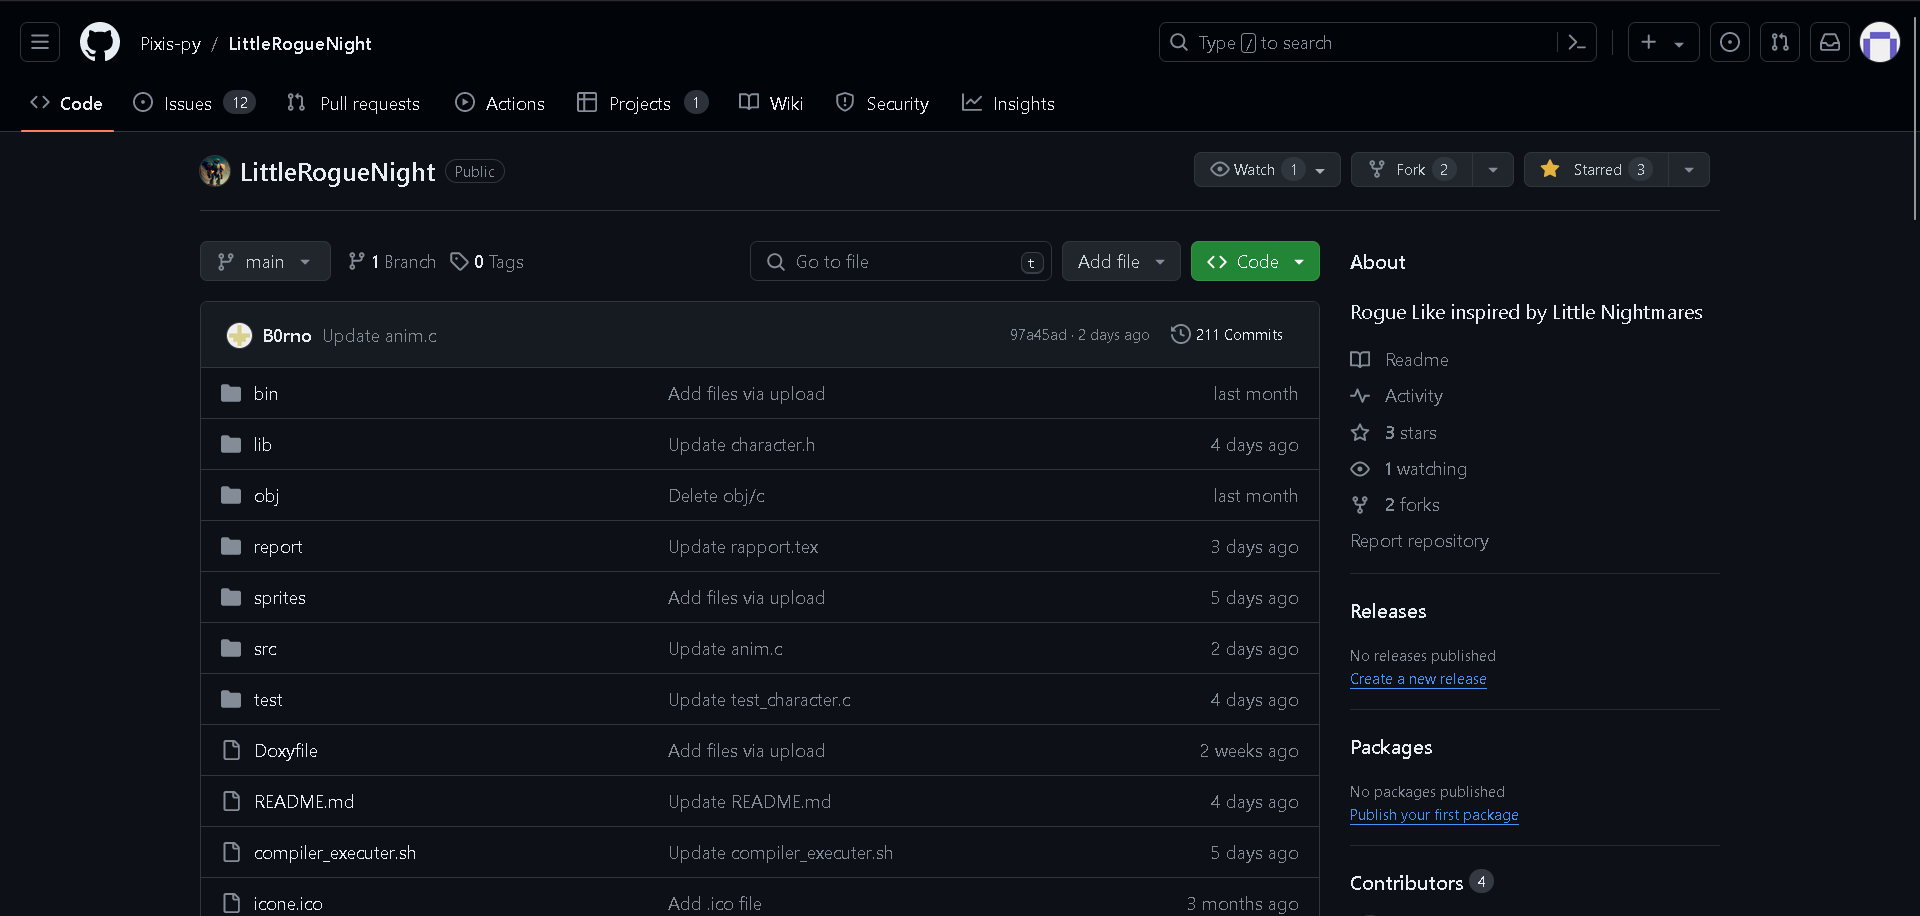
\includegraphics[width=12cm]{Github.png}
\caption{Répartition des dossiers comme sur Visual Studio Code mais sous Github}
\label{fig4}\\
\end{center}
Parallèlement, un \gls{Trello} est utilisé pour représenter le cahier des charges et suivre l'avancement des fonctionnalités. Des checklists ont été créées pour chaque tâche, permettant à chaque membre de l'équipe de suivre sa progression et de s'assurer que les objectifs sont atteints en temps voulu.\\
\begin{center}
\centering
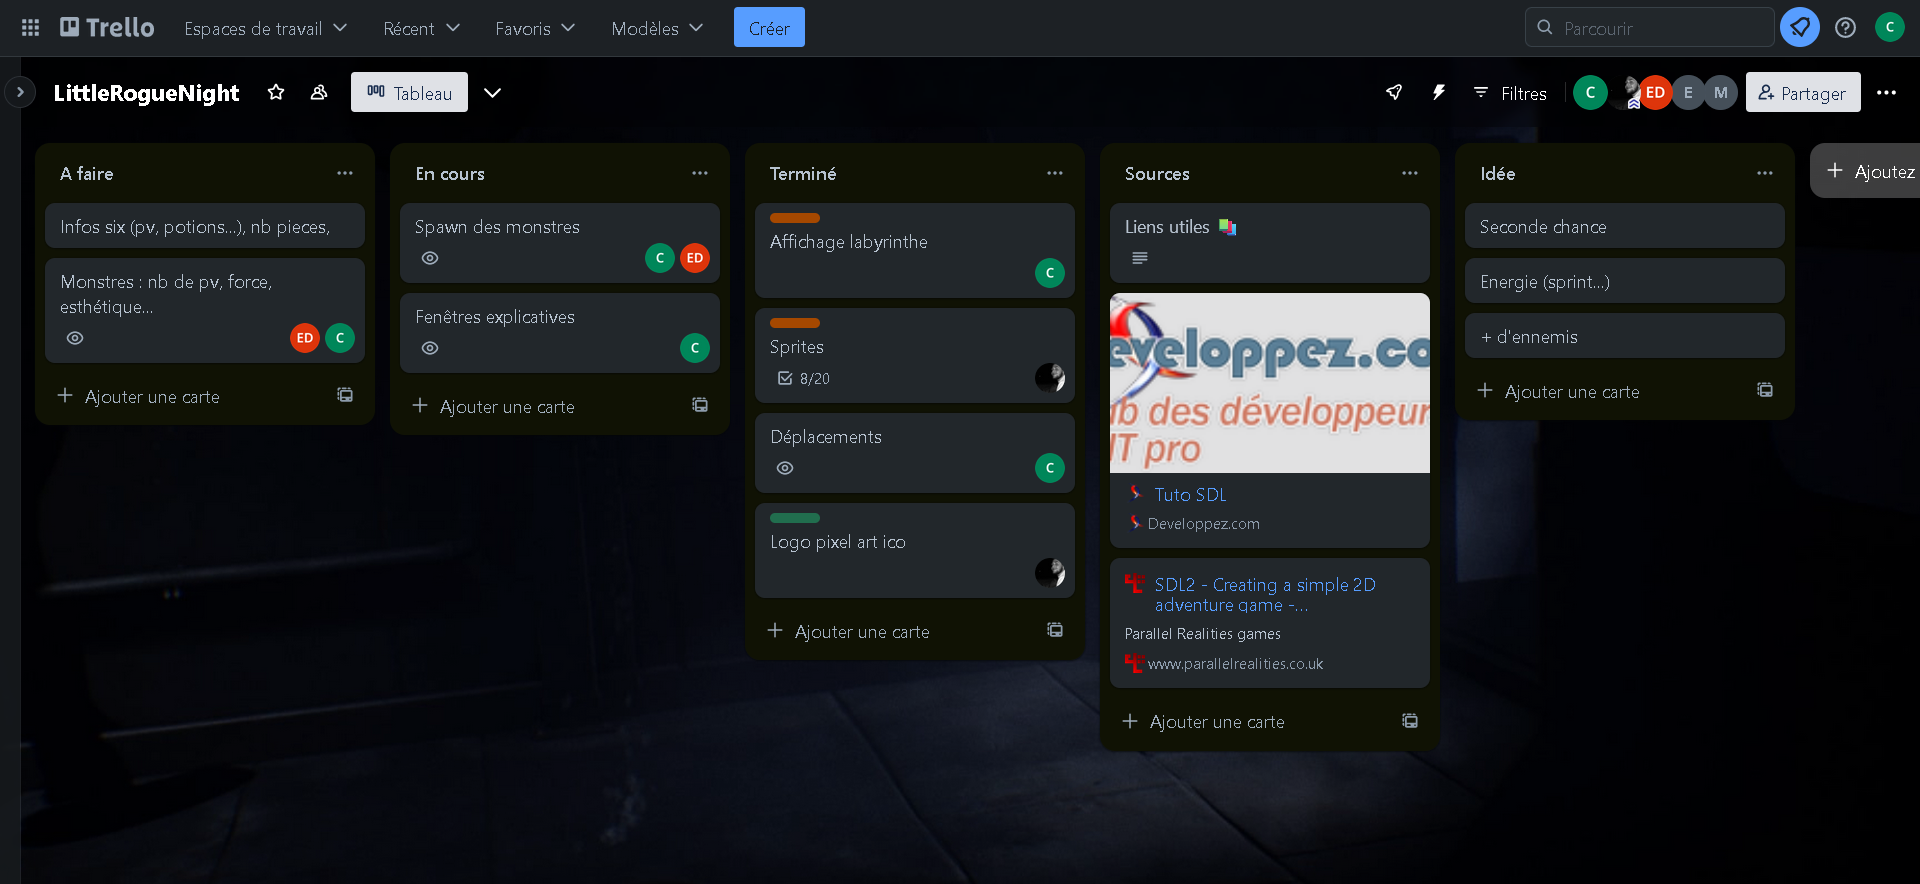
\includegraphics[width=12cm]{Trello.png}
\caption{Répartition des tâches entre les membres de l'équipe}
\label{fig4}\\
\end{center}
En outre, au début du projet, nous avons également utilisé un Drive Google pour partager des documents et des ressources nécessaires à la planification et au démarrage du projet. Ce Drive a notamment été utile pour stocker des documents de référence, des captures d'écran de l'avancée du projet pour les premiers affichages du labyrinthe et d'autres fichiers partagés entre les membres de l'équipe, offrant ainsi un espace de stockage centralisé et accessible à tous.\\

L'utilisation combinée de ces outils a grandement contribué à la gestion efficace du projet, en facilitant la collaboration, le suivi de l'avancement et la gestion des ressources, tout en favorisant une communication transparente et une coordination harmonieuse entre les membres de l'équipe.

Nous avons également utilisé une gamme d'outils spécifiquement sélectionnés pour faciliter le processus de création et garantir la qualité du produit final.
\textbf{Environnement de développement intégré (IDE) : Visual Studio Code} :
L'IDE joue un rôle crucial dans notre processus de développement. Nous avons choisi Visual Studio Code pour sa polyvalence et sa facilité d'utilisation. L'interface intuitive de Visual Studio Code nous a permis d'écrire, de modifier et de déboguer notre code de manière efficace. De plus, l'intégration d'extensions a considérablement amélioré notre flux de travail. Parmi ces extensions, l'outil \textit{\gls{doxygen}} revêt une importance particulière.

\textbf{Extension Doxygen pour la documentation} :
L'extension Doxygen pour Visual Studio Code a été un atout majeur dans la production de la documentation de notre projet. Cette extension simplifie le processus de documentation en permettant la génération de commentaires Doxygen quasiment automatiquement. Grâce à des balises prédéfinies telles que "/// @brief" ou "/// @param", nous avons pu documenter efficacement notre code, facilitant ainsi sa compréhension et sa maintenance ultérieure.
\begin{center}
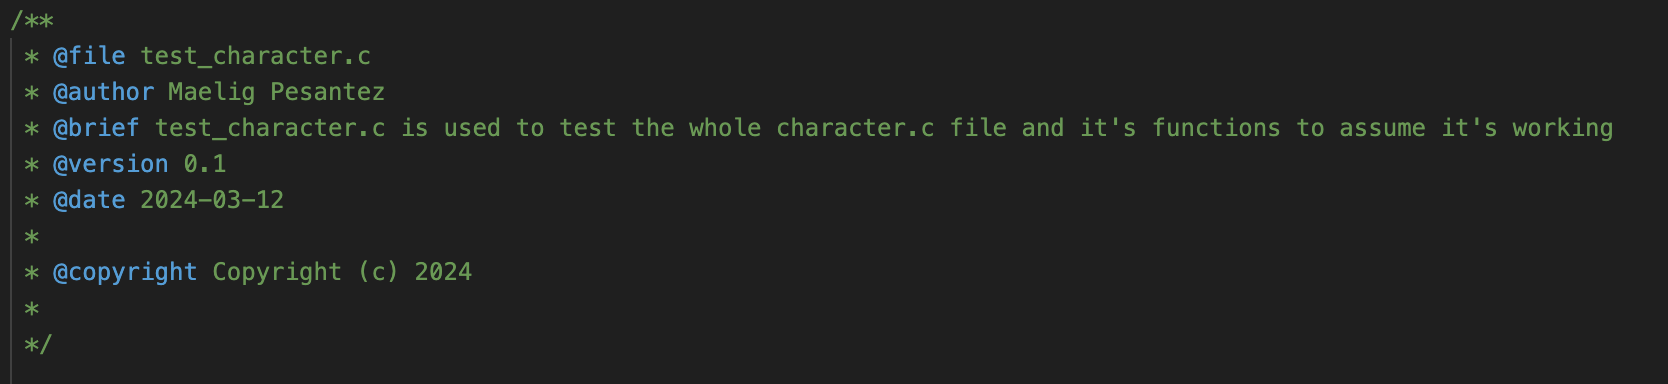
\includegraphics[width=10cm]{doxygen.png}\\
\caption{{\emph{Exemple d'un commentaire doxygen généré automatiquement}}}
\label{fig8}\\
\end{center}
\begin{center}

\textbf{Tests unitaires avec CUnit} :
Pour garantir la fiabilité et la robustesse de notre code, nous avons intégré des tests unitaires à notre processus de développement. Pour cela, nous avons utilisé la bibliothèque \textit{\gls{cunit}}, largement reconnue dans l'écosystème du langage C pour sa capacité à effectuer des tests unitaires efficaces. Ces tests ont été conçus pour évaluer le bon fonctionnement de nos fichiers sources contenant des structures cruciales, assurant ainsi la qualité du code avant son intégration. 
\begin{center}
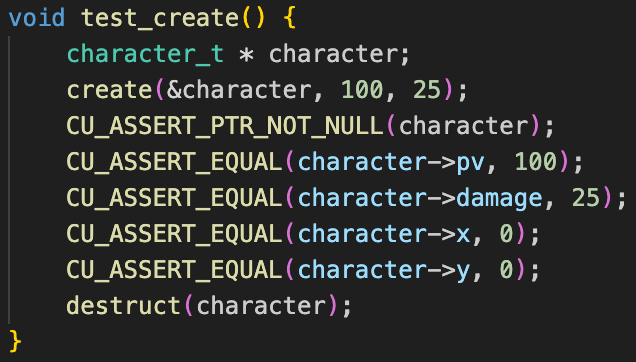
\includegraphics[width=10cm]{create.png}\\
\caption{{\emph{Exemple d'une fonction de test: creation d'un character}}}
\label{fig6}\\
\end{center}
\begin{center}
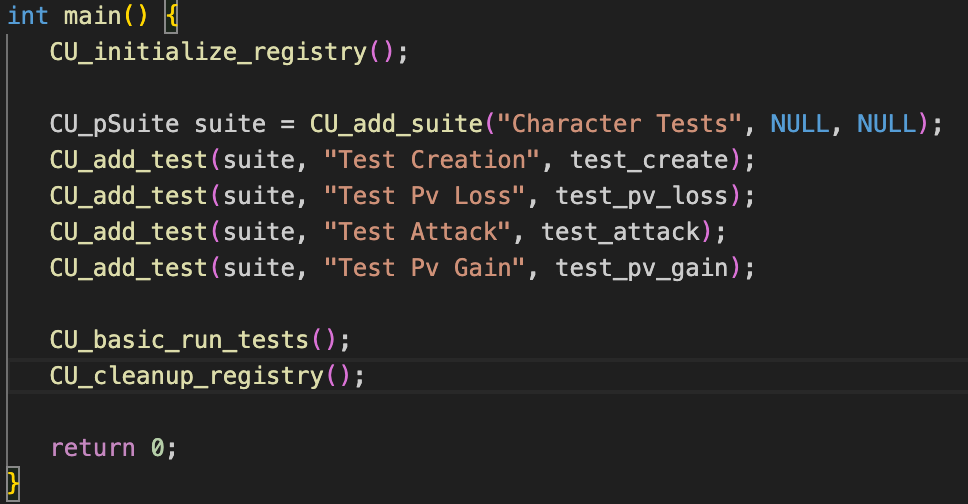
\includegraphics[width=10cm]{maincunit.png}\\
\caption{{\emph{Fonction main d'un test unitaire: appel des fonctions de test de la structure character}}}
\label{fig7}\\
\end{center}
\begin{center}
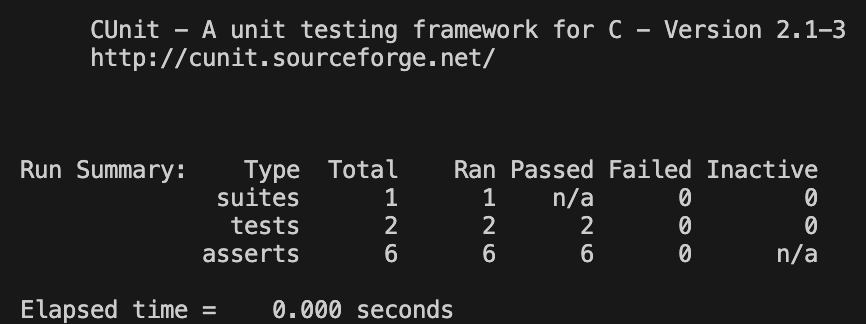
\includegraphics[width=10cm]{cunit.png}\\
\caption{{\emph{Sortie du test unitaire de la structure character et de ses fonctions}}}
\label{fig5}\\
\end{center}

\textbf{Production de sprites avec Piskel} :
Bien que cela ne soit pas directement lié au développement du jeu en lui-même, il est important de mentionner l'outil Piskel que nous avons utilisé pour produire les sprites de LittleRogueNight. Piskel est un outil de pixel art en ligne gratuit qui nous a permis de créer des sprites uniques et personnalisés pour notre jeu, contribuant ainsi à son esthétique et à son identité visuelle.\\
\begin{center}

\includegraphics[width=12cm]{six_run.png}\\
\caption{{\emph{Exemple de spritesheets avec l'animation de marche de six}}}
\label{fig4}\\
\end{center}

\subsection{Rôles}
Concernant les tâches, Maëlig est en charge de la création des \textit{\gls{spritesheets}}, qui représentent toutes les images nécessaires à l'animation des entités du jeu. Pour ce faire, il utilise un logiciel en ligne puis intègre ces animations dans le code. Outre cette responsabilité, Maëlig prend en charge la gestion des combats entre le héros Six et les concierges (monstres provenant du jeu originel) présents dans le labyrinthe. Il est également responsable du "spawn" (apparition) des entités au sein du labyrinthe, garantissant ainsi une expérience de jeu fluide et dynamique.

Ensuite, Enzo se concentre sur l'affichage du menu principal ainsi que des menus annexes, en mettant en place les boutons et en assurant la gestion de la souris pour l'interaction utilisateur. Il contribue également à l'apparition aléatoire des entités dans le labyrinthe, ajoutant ainsi une dimension aléatoire au jeu qui enrichit l'expérience du joueur.

Enfin, Clément prend en charge la création et l'affichage du labyrinthe, une tâche cruciale pour l'immersion du joueur dans l'environnement du jeu. Il développe également les mécanismes de déplacements et de collisions des entités, assurant ainsi le réalisme et la cohérence du monde virtuel. Clément apporte également son expertise au codage de la partie combat, collaborant avec Maëlig et Enzo pour garantir son bon fonctionnement. En outre, il est responsable de l'affichage des fenêtres d'explications au début du jeu, fournissant ainsi au joueur les informations nécessaires pour commencer son aventure de manière informée et engagée.

\section{Conception}
\subsection{Analyse et cahier des charges}
Les règles du jeu s'articulent autour du personnage principal, Six, qui doit naviguer à travers un \gls{labyrinthe} complexe en quête de la sortie, située en bas à droite de la structure. Au cours de cette progression, Six est confronté à une multitude d'\gls{ennemis} qu'il doit soit éviter, soit affronter.

Pour se défendre, Six dispose d'attaques. Au 1er niveau, il a recours aux \gls{drifts}. Aux niveaux 2 et 3, il obtient également un \gls{briquet}, une arme plus efficace pour tuer ses adversaires.

La survie du joueur dépend de sa capacité à gérer ses vies limitées. Il peut régénérer ces dernières en collectant des morceaux de viande et des potions dispersés dans le labyrinthe. Cette gestion prudente des ressources est cruciale pour affronter les dangers croissants qui ponctuent sa progression.

La difficulté s'intensifie au fil des niveaux, notamment avec les \gls{concierges}, les monstres des niveaux. Leur résistance et leur puissance augmentent progressivement, accentuant le défi pour le joueur. Parallèlement, l'architecture du labyrinthe évolue, passant d'une structure en terre, puis en bois et pour finir des murs de briques aux niveaux supérieurs. Cette transition visuelle reflète la complexité croissante du défi et contribue à l'immersion du joueur dans l'univers du jeu.
\begin{center}
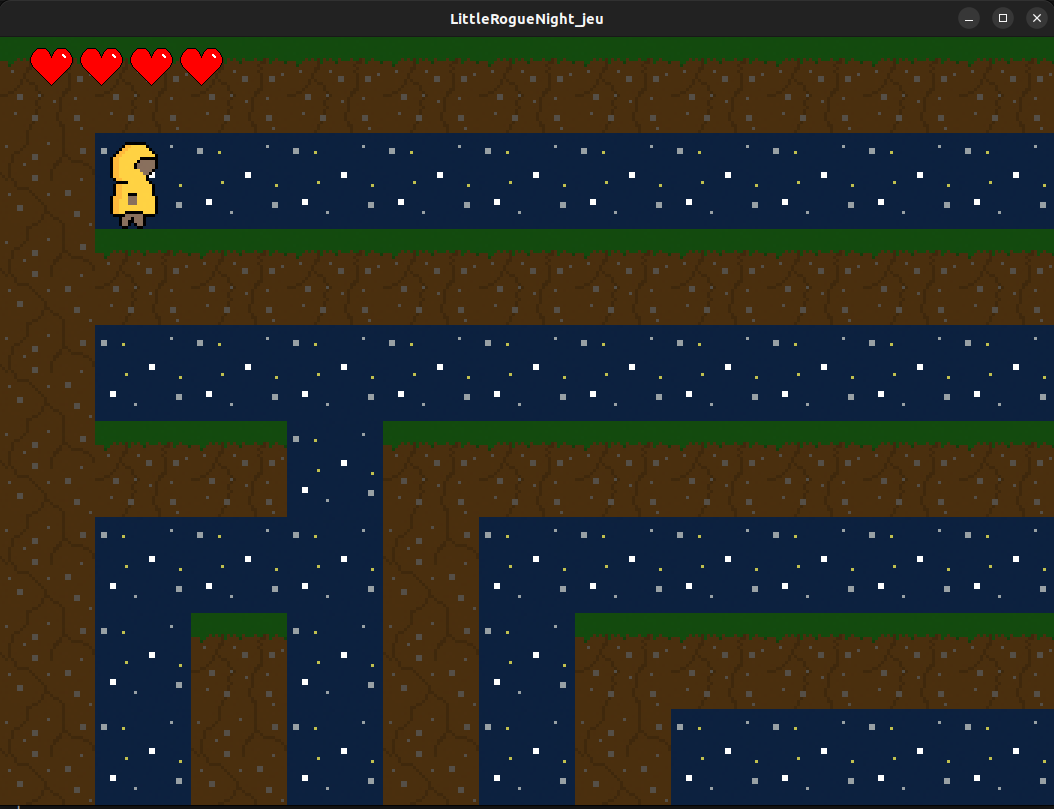
\includegraphics[width=5.5cm]{niveau_un.png}
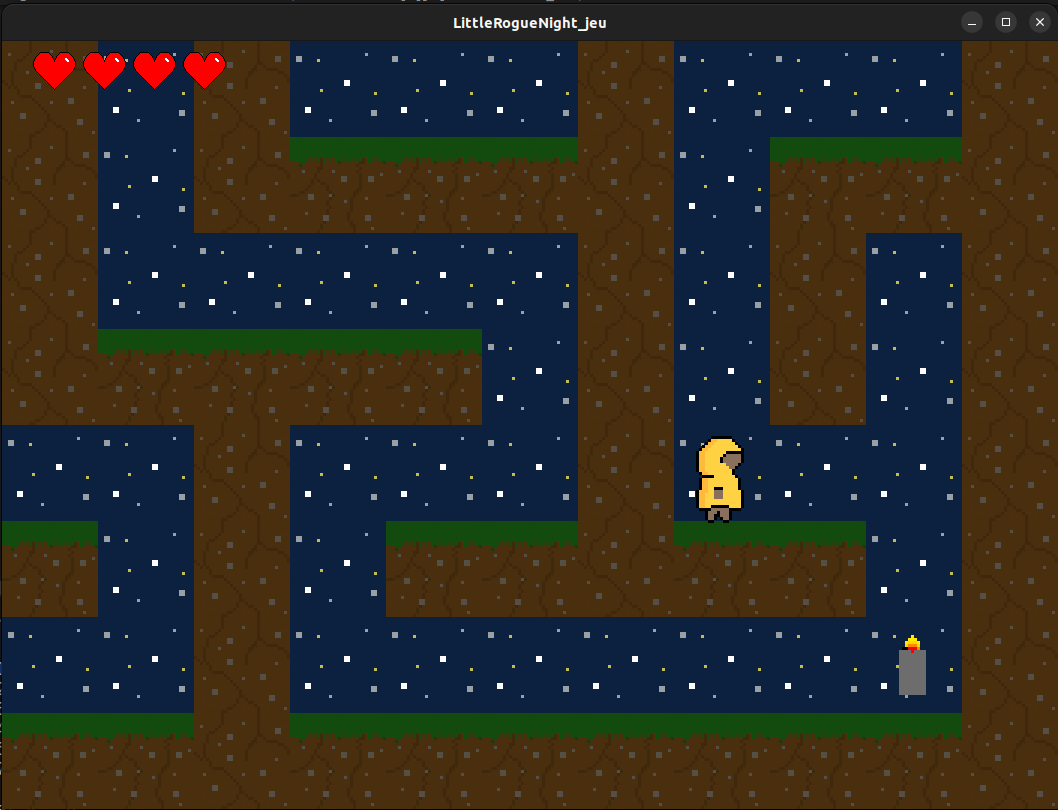
\includegraphics[width=5.5cm]{fin_niveau_un.png}
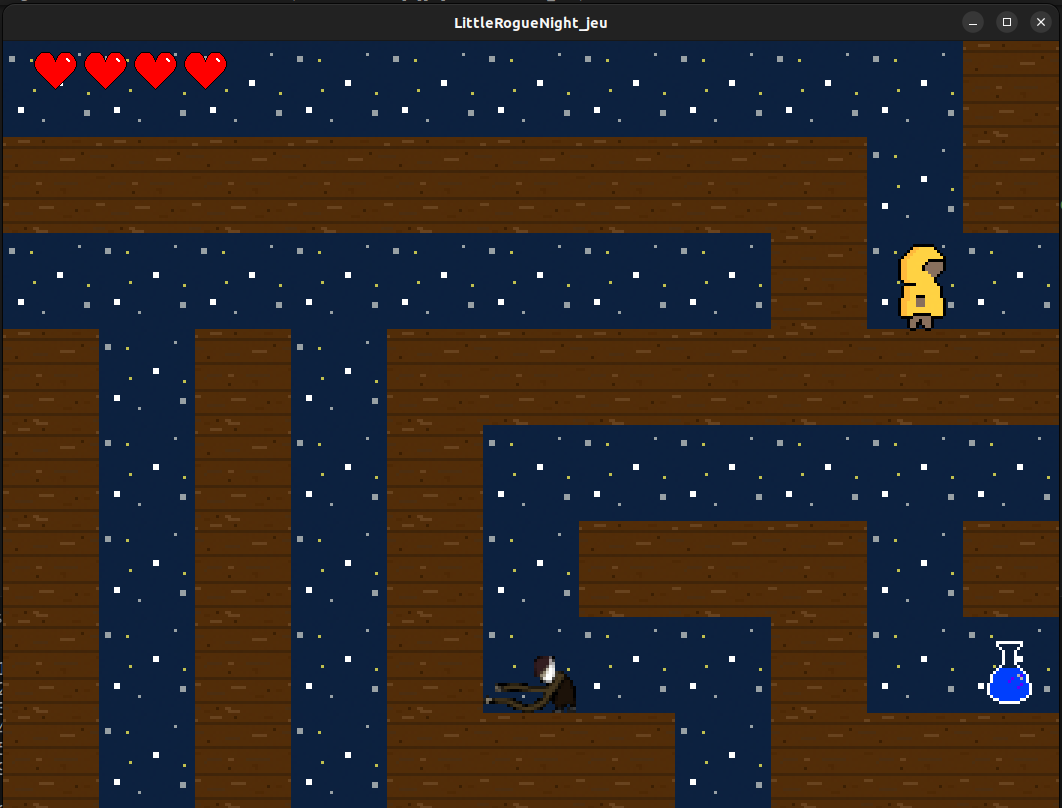
\includegraphics[width=5.5cm]{potion_et_monstre.png}
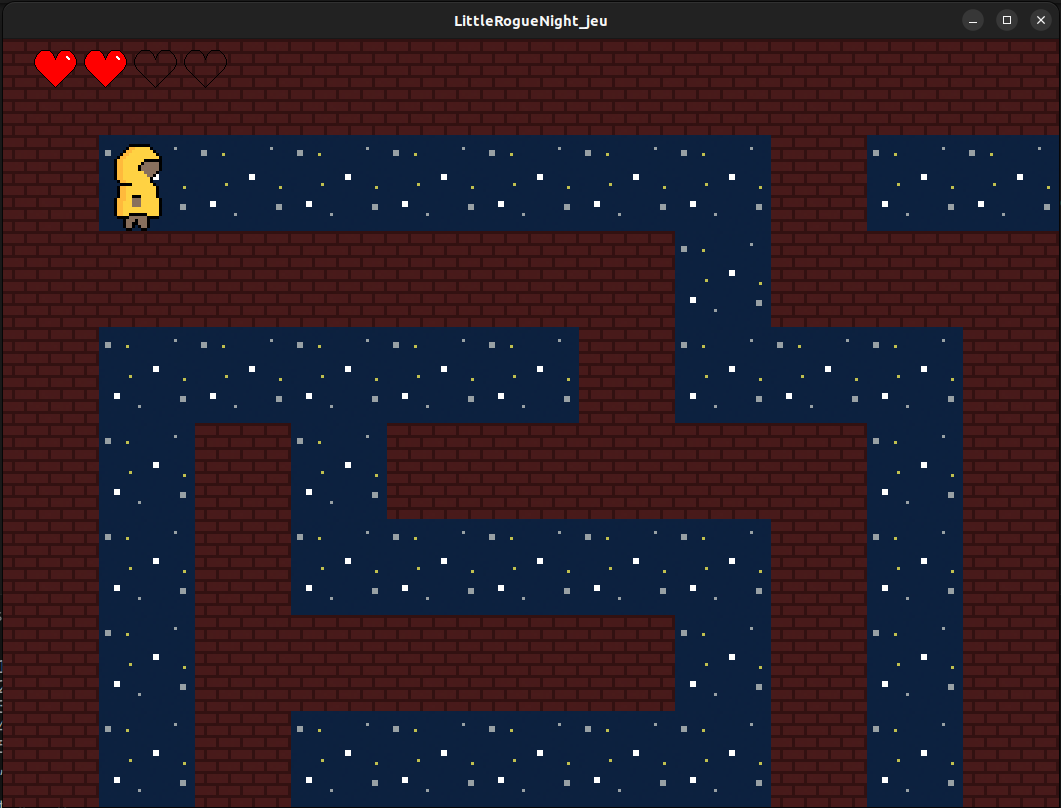
\includegraphics[width=5.5cm]{niveau_trois.png}

\label{fig4}\\
\end{center}

\clearpage
\section{Développement}
   \subsection{Fonctionnemeent des algorithmes}
   Pour la création du \gls{labyrinthe} parfait, Clément utilise la génération aléatoire, avec des \gls{piles} et des \gls{files}, rencontrée au semestre 3 en Algorithmique et Programmation 2.
   Bien sûr, les fonctions ont été légèrement modifiées pour s'adapter à nos fins : la gestion des différentes tuiles grâce à des \gls{constantes} comme NUIT, TERRE, TERREVERTE etc, les paramètres de la fonction d'affichage changent pour permettre d'afficher le labyrinthe directement sur le \gls{rendu}  grâce à des rectangles (SDL\_Rect) qui se "posent" sur le rendu. 
   \\
    \begin{center}
        \centering
        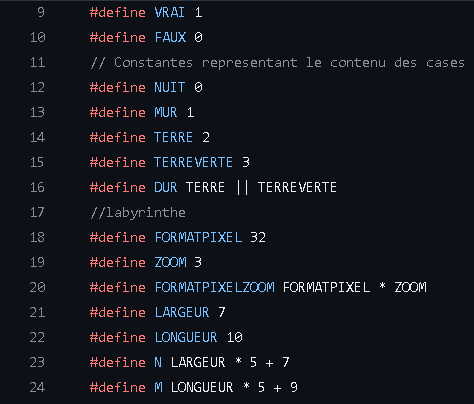
\includegraphics[width=12cm]{lab_h.png}
        \caption{Constantes du labyrinthe}
        \label{fig4}\\
    \end{center}
   La fonction permet également de rendre le labyrinthe plus esthétique en mettant un bloc de terre avec de l'herbe au dessus des autres blocs de terre dans le niveau 1 et le labyrinthe est également réparti en plusieurs parties qui sont décalées en fonction des variables coeffX et coeffY : si le joueur arrive à une certaine distance près d'un bord de l'écran, alors le coeff concerné est incrémenté ou décrémenté selon les circonstances et donc tout est décalé dans l'affichage du labyrinthe.\\
   \begin{center}
        \centering
        \includegraphics[width=5.5cm]{defilement_un.png}
        \includegraphics[width=5.5cm]{defilement_deux.png}
        \caption{Défilement du labyrinthe et décalage de Six}
        \label{fig4}\\
    \end{center}
   
   
   
   Le niveau 2 est constitué de tuiles de bois et le niveau 3 affiche des briques. \\Maintenant, la partie animation du jeu aborde plusieurs fonctionnalités :\\
   -Les monstres deviennent de plus en plus puissants quand Six avance en terme de niveau de labyrinthe\\
   -Pour la détection des touches, il faut simplement déterminer si le joueur appuie sur une touche nécessaire au jeu, ce qui met à 1 la variable concernée et idem si la touche est relâchée. Cependant, une distinction se fait quant aux directions : si la dernière touche appuyée puis relâchée est 'd' par exemple, alors Six regarde vers la droite et idem pour la gauche.\\
   -Chaque touche est reliée à un affichage différent du sprite et des combinaisons peuvent être utilisées, ainsi si Six avance à droite grâce à la touche 'd' et qu'il saute en même temps par la touche "espace", alors cela fait appel à 2 animations. Pour coder cela, il faut créer une boucle for avec autant de répétitions qu'il y a d'images dans le spritesheet d'animation, par exemple, pour courir, 11 images ont été créées par Maëlig et chaque d'entre elles possède une position en x différente. Pour appliquer un zoom sur chaque image, la constante FORMATPIXELZOOM est utilisée car elle représente le format 32 pixels des images multiplié par le zoom, ici 3, pour obtenir des images de 96 pixels. \\
   -Concernant les positions des entités présentes dans le labyrinthe, chacune d'entre elles possède des coordonnées et un nouveau SDL\_Rect associé au nom (souvent utilisé "position\_nom\_sprite") permettant de manipuler leurs coordonnées en contrôlant qu'elles respectent certaines conditions : elles ne doivent pas dépasser la fenêtre et apparaître quand il le faut grâce aux décalages par les coeffX et coeffY. Cela se fait par un calcul de la position dans le labyrinthe par rapport aux pixels : on divise cette valeur par FORMATPIXELZOOM et encore par 9, qui correspond à ZOOM². Cependant, il y a un petit décalage selon la direction de Six : s'il regarde à droite alors il faut ajouter 8 à la position initiale et 70 s'il regarde à gauche. Pour l'opétation inverse, pour effectuer l'apparition aléatoire des entités dans le labyrinthe, on multiplie la valeur par FORMATPIXELZOOM et on effectue le décalage en soustrayant par le coeff correspond multiplié par FORMATPIXELZOOM.\\
   -Pour appliquer la gravité, il faut simplement vérifier que la case sur laquelle se trouve Six est de type NUIT auquel cas il tombe jusqu'à ce que ce ne soit plus le cas. C'est presque le même système pour les sauts sauf que le y manipulé sur la position de l'entité est décrémenté à la place d'être incrémenté pour la gravité.\\
   -A la fin d'un niveau, Six est téléporté au début du niveau suivant s'il y en a un autre, sinon une fenêtre apparait lui demandant s'il veut retourner au menu, arrêter de jouer ou encore poursuivre le jeu en débutant du niveau souhaité. Il obtient alors, bien sûr, tous ses points de vie en début de partie.\\
   -Maintenant, s'il finit par mourir au cours d'un niveau, il revient au début du niveau 1 avec tous ses points de vie et perdant ainsi toute son avancée dans le jeu ! Toutes les entités sont de nouveau placés aléatoirement.\\
   -Pour tuer un monstre ou consommer une potion de points de vie ou de la viande, 3 variables ont été créées : si l'une d'entre elle vaut 1 alors l'entité concernée disparaît de l'écran.\\
   -Enfin, une détection de Six par les entités est nécessaire au bon fonctionnement du jeu : s'il se trouve à moins de 2 blocs du monstre et qu'il n'attaque pas, donc il ne drift pas, alors il reçoit des dégâts toutes les 0.75 secondes (1 seconde est trop long), s'il attaque par contre et qu'il est toujours à la même distance alors c'est le monstre qui reçoit des dégâts. Idem pour la potion, seulement, s'il a tous ses points de vie, alors la potion reste dans le labyrinthe. EXEMPLE MORT ET RESPAWN ?
\clearpage   
   \subsection{Structures}

En langage C, diverses \gls{structures} sont utilisées dans les fichiers du jeu, notamment les files et les piles. Ces structures jouent un rôle important en matière de stockage des données, offrant des solutions efficaces pour gérer la manipulation des informations. Les piles et les files, couramment employées en programmation, présentent des caractéristiques distinctes avec des avantages et des inconvénients spécifiques. Tant les piles que les files possèdent une tête (représentant le premier élément de la liste) ainsi qu'une queue (le dernier élément de la liste).
\\\\
\begin{center}
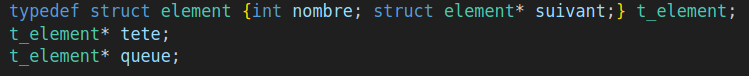
\includegraphics[width=12cm]{file.png}\\
\caption{{\emph{Structure file}}}
\label{fig1}\\
\end{center}
\begin{center}
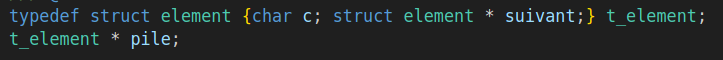
\includegraphics[width=12cm]{pile.png}\\
\caption{{\emph{Structure pile}}}
 \label{fig2}\\
 \end{center}
Les piles sont des structures dans lesquelles on peut uniquement ajouter des éléments par la tête et retirer des éléments également par la tête (opérations d'empilement et de dépilement). En revanche, les files permettent l'ajout d'éléments par la tête et leur retrait par la queue (opérations d'enfilement et de défilement).

L'utilisation de piles et de files en langage C facilite la gestion efficace des données, notamment pour la manipulation des matrices. Dans le contexte du jeu, cela simplifie la création et la manipulation du labyrinthe, permettant un fonctionnement fluide et optimisé des mécanismes de jeu.

La structure \textit{\gls{character}} prend en charge les différentes entités présentes dans le jeu telles que le personnage contrôlé par le joueur, les monstres, ainsi que les objets comme les potions. Cette structure offre une abstraction pratique pour représenter les éléments interactifs du jeu, facilitant ainsi la gestion des interactions entre eux et avec l'environnement du jeu.
\begin{center}
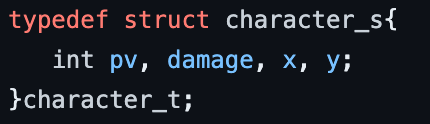
\includegraphics[width=11cm]{character.png}\\
\caption{{\emph{Structure character}}}
\label{fig3}\\
\end{center}


\subsection{Fichiers}

Les fichiers ont été organisés de la même manière que sur le Github, c'est à dire en gèrant chaque aspect du jeu de manière efficace, en les rangeant dans différents dossiers en fonction de leur type et leur fonctionnalité. Cette structuration nous a permis de maintenir un code propre et bien organisé tout au long du développement.

Dans le dossier \textit{src}, nous avons regroupé tous les fichiers contenant du code source écrit en langage C. Cette section constitue le cœur du projet, abritant les implémentations des fonctionnalités principales du jeu, telles que la logique de jeu, la gestion des personnages et des niveaux.

Le dossier \textit{bin} contient l'exécutable du jeu ainsi que les fichiers de test associés. Ces fichiers de test sont essentiels pour vérifier la robustesse et la fiabilité de notre code, en s'assurant que toutes les fonctionnalités répondent aux exigences spécifiées.

Le répertoire \textit{lib} héberge les fichiers d'en-tête contenant les prototypes de fonctions, les définitions de structures et les constantes utilisées dans notre code source. Cette section joue un rôle crucial dans l'organisation et la documentation de notre projet, en fournissant une référence claire pour toutes les fonctions et structures implémentées et elle est primordiale pour l'édition de liens de la compilation du programme par le makefile.

Le dossier \textit{obj} contient les fichiers objets générés lors de la compilation du code source. Ces fichiers objets sont essentiels pour créer l'exécutable final du jeu, en regroupant toutes les parties du code source en un seul programme exécutable.

Le répertoire \textit{sprites} est subdivisé en plusieurs sections, chacune contenant les différents sprites nécessaires à l'affichage du jeu. Les \textit{\gls{sprites}}, qui représentent des images en deux dimensions pouvant être déplacées indépendamment du décor de l'affichage, sont essentiels pour créer une expérience visuelle immersive et attrayante pour les joueurs.

Enfin, le dossier \textit{test} abrite tous les fichiers de test des fonctions, garantissant qu'elles fonctionnent correctement et ne produisent pas d'erreurs inattendues. Ces tests jouent un rôle crucial dans la validation et la vérification de la qualité du code, en s'assurant que toutes les fonctionnalités du jeu répondent aux normes spécifiées.

\clearpage
\section{Conclusion}

Le projet LittleRogueNight a atteint ses objectifs fixés en termes de fonctionnalités de base. Le jeu est fluide, ce qui peut être difficile à mettre en place au vu de la gestion de la mémoire de la \gls{sdl} et du nombre de \gls{sprites} présents sur l'écran. La partie recherche du chemin vers la fin du labyrinthe fait son effet grâce au principe du labyrinthe parfait. La détection du héros par les ennemis est fonctionnelle : en suivant un système de déplacement simple et de spawn aléatoire, on obtient des monstres sans \gls{ia} qui ne restent pas immobiles. Les collisions et la gravité ont également été ajoutées comme prévu et fonctionnent bien. Les menus ont été implémentés conformément aux spécifications, offrant une navigation intuitive en dehors du jeu. Cependant, des fonctionnalités supplémentaires, telles que des spécificités pour les ennemis et les niveaux comme des pièges, le fait de détruire certains blocs, d'autres ennemis ayant des attaques différentes, n'ont pas pu être implémentées en raison de contraintes temporelles et par l'abandon d'un des membres de l'équipe. \\
Les éléments prévus mais non réalisés, tels que des passages secrets, des salles spéciales et un magasin et donc un système d'argent, auraient pu ajouter de la variété et de l'intérêt au jeu. Cependant, ils auraient demandé de trop grosses modifications de l'algorithme de génération du labyrinthe et nous avons décidé de nous concentrer sur des fonctionnalités de base pour obtenir un jeu fonctionnel. D'autre part, l'ajout de niveaux supplémentaires aurait renforcé la durée de vie et la richesse du \gls{gameplay}. Enfin, offrir au joueur des "pouvoirs" spéciaux tels que l'invisibilité ou la téléportation, avec un système de \gls{cooldown}, aurait permis d'ajouter une dimension stratégique et tactique au jeu. L'idée de système de récompenses à la fin de chaque niveau aurait pu apporter un côté intéressant au jeu et le joueur serait plus enjoué à vouloir continuer à progresser. 

Le projet LittleRogueNight, malgré quelques lacunes, se distingue comme une réalisation robuste et fonctionnelle, offrant une expérience de jeu gratifiante. Cette étude permet d'entretenir une évaluation positive de ce projet, qui a représenté l'un des premiers efforts collaboratifs de l'équipe de recherche. Contrairement aux pratiques usuelles observées dans le développement de logiciels individuels, la mise en place de ce projet a exigé l'adoption de nouveaux protocoles de travail et d'outils tels que GitHub et des solutions de gestion de projet. En outre, celui-ci a permis de mettre en œuvre les compétences informatiques acquises au cours des 2 premières années d'études universitaires en informatique, favorisant ainsi le développement de compétences en programmation et en conception de jeux vidéos au sein de l'équipe.

\clearpage

\section{Glossaire}
\printglossary

\end{document}
